%%%%%%%%%%%%%%%%%%%%%%%%%%%%%%%%%%%%%%%%%
% NIH Grant Proposal for the Specific Aims and Research Plan Sections
% LaTeX Template
% Version 1.0 (21/10/13)
%
% This template has been downloaded from:
% http://www.LaTeXTemplates.com
%
% Original author:
% Erick Tatro (erickttr@gmail.com) with modifications by:
% Vel (vel@latextemplates.com)
% Michael ma2196@columbia.edu
% with assistance from Jonah G.
% Adapted from:
% J. Hrabe (http://www.magalien.com/public/nih_grants_in_latex.html)
%
% License:
% CC BY-NC-SA 3.0 (http://creativecommons.org/licenses/by-nc-sa/3.0/)
%
%%%%%%%%%%%%%%%%%%%%%%%%%%%%%%%%%%%%%%%%%

%----------------------------------------------------------------------------------------
%	PACKAGES AND OTHER DOCUMENT CONFIGURATIONS
%----------------------------------------------------------------------------------------

\documentclass[11pt,notitlepage]{article}

% A note on fonts: As of 2013, NIH allows Georgia, Arial, Helvetica, and Palatino Linotype. LaTeX doesn't have Georgia or Arial built in; you can try to come up with your own solution if you wish to use those fonts. Here, Palatino & Helvetica are available, leave the font you want to use uncommented while commenting out the other one.

\usepackage[super]{natbib}
\usepackage{palatino} % Palatino font
%\usepackage{helvet} % Helvetica font
\renewcommand*\familydefault{\sfdefault} % Use the sans serif version of the font
\usepackage[T1]{fontenc}
\linespread{1.05} % A little extra line spread is better for the Palatino font
\usepackage{hyperref} % to allow hyperlinks to websites on the internet
\usepackage[hypcap]{caption} % to point to the top of the image
\usepackage{lipsum} % Used for inserting dummy 'Lorem ipsum' text into the template
\usepackage{amsfonts, amsmath, amsthm, amssymb} % For math fonts, symbols and environments
\usepackage{graphicx} % Required for including images
\usepackage{booktabs} % Top and bottom rules for table
\usepackage{wrapfig} % Allows in-line images
\usepackage[labelfont=footnotesize]{caption} % Make figure numbering in captions bold
\usepackage[top=0.5in,bottom=0.5in,left=0.5in,right=0.5in]{geometry} % Reduce the size of the margin
\pagestyle{empty} % Remove page numbers

\hyphenation{ionto-pho-re-tic iso-tro-pic fortran} % Specifies custom hyphenation points for words or words that shouldn't be hyphenated at all

  
  % to reduce white space between PARAGRAPHS
\setlength{\parskip}{0pt}
\setlength{\parsep}{0pt}

  % additional parameters
%\setlength{\headsep}{0pt}
%\setlength{\topskip}{0pt}
%\setlength{\topmargin}{0pt}
%\setlength{\topsep}{0pt}
%\setlength{\partopsep}{0pt}

  % to reduce white space around figures
% \setlength{\textfloatsep}{0pt plus 0pt minus 0pt}

  % to reduce white space between SECTIONS
\usepackage[compact]{titlesec}
\titlespacing{\part}{0pt}{5pt}{4pt}
%\titlespacing{\subsection}{0pt}{*0}{*0}
%\titlespacing{\subsubsection}{0pt}{*0}{*0}
%\titlespacing{\subparagraph}{0pt}{*0}{*0}
\titlespacing*{\subparagraph} {\parindent}{1ex plus 1ex minus .2ex}{0.5em}


\begin{document}


%----------------------------------------------------------------------------------------
%	SPECIFIC AIMS
%----------------------------------------------------------------------------------------
\part*{Specific Aims}
Acute respiratory failure (ARF) requiring mechanical ventilation is common in hospitalized patients; prolonged mechanical ventilation often leads to multi-organ failure. We will model electronic medical record (EMR) and pragmatic clinical trial data to predict and to prevent acute severe respiratory failure in hospitalized patients.

\textbf{Severe acute respiratory failure (ARF) requiring mechanical ventilation leads to increased mortality,} increased cognitive and functional impairment. EMR surveillance can identify hospitalized patients at risk, days before their deteriorating conditions are typically recognized; earlier initiation of preventive interventions can reduce morbidity, mortality and expenses: My mentor Dr. Gong is leading a two phase pragmatic clinical trial: APPROVE, phase 1, develops a classical algorithm to identify patients at risk; PROOFCheck, phase 2, aims to improve outcomes by triggering a prevention checklist targeting those patients, the APPROVE algorithm identifies. 

\textbf{Hierarchical modeling may be transformative for EMR-based prediction and prevention} and exploit the nested hierarchical granularity typical for EMRs. We propose to fit a more sophisticated hierarchical prediction algorithm than currently developed in APPROVE; we propose (a) to allow model parameters to vary between patients, medical floors, services or institutions and (b) to model temporal effects, e.g. seasonal effects, shifting population characteristics or heterogeneous provider behavior which might otherwise limit prediction accuracy. Incomplete clinical data limit prediction algorithms, but are characteristic for EMRs. I will develop new data imputation algorithms using auxiliary data, a novel approach to overcome issues with missing at random assumptions. 

\textbf{Hierarchical models improve prediction over classical approaches owing to additional information}, gained from (a) modeling the rich spatial and temporal organization of EMRs more realistically, (b) imputing incomplete data from auxiliary data and (c) partial pooling. Patients treated by the same team, in similar settings will show similar clinical trajectories and responses. Partial pooling will improve precision and accuracy by informing parameter estimates with data from all other patients, using information from different but related subsets, especially in subgroups with sparse data. The near real-time \textit{integration} of auxiliary data imputation and hierarchical modeling with partial pooling into one coherent EMR-surveillance model is groundbreaking. 

\textbf{Novel algorithms push the envelope of computability for Bayesian prediction models.} We choose Bayesian inference, novel for EMR prediction, for its flexibility in hierarchical modeling. Computational implementation can be challenging. My co-mentor Dr. Gelman is leading the NSF-funded development of the probabilistic programming language Stan. His novel algorithm achieves much faster model convergence and parameter estimation. My second co-mentor Dr Hall is also a seasoned Bayesian statistician. He will supervise me for clever statistical formulation or transformation to further push the boundaries of computability for large EMRs. My exceptional and multidisciplinary team of mentors is lead by Dr. Gong with her clinical angle on Big Data science. Together, we will integrate innovative approaches to data imputation with advanced hierarchical prediction models to form a near real-time EMR-based clinical decision tool with practical utility in critical care.  The integration of pioneering statistical modeling with pragmatic clinical EMR-surveillance constitutes our unique innovation.
\vspace{-5pt}
\begin{flushleft}
\textbf{Hypothesis:} \textit{Compared to classical approaches, joint hierarchical Bayesian models improve prediction, prevention and compliance analysis in a pragmatic trial to prevent respiratory failure in hospitalized patients.}
\end{flushleft}
\vspace{-5pt}
\textbf{Specific aims}
\vspace{-5pt}
\begin{flushleft}
\textbf{Aim 1: To improve incomplete data imputation and early prediction of acute respiratory failure.}
\end{flushleft}
\vspace{-8pt}

\textit{SA 1a:} To build a pragmatic EMR-based hierarchical Bayesian model implemented in the ultra-fast statistical software Stan to predict a composite outcome [death or prolonged mechanical ventilation > 48 hours] in inpatients.

\textit{SA 1b:} To further develop Bayesian data imputation algorithms of missing clinical data using auxiliary data, to identify auxiliary measure properties (ceiling, floor and threshold effects), to integrate imputation and prediction in one coherent hierarchical Bayesian model and to assess the  predictive performance  compared to the classical algorithm by Dr. Gong by the area under the curve (AUC) of their receiver operating characteristics (ROC).

\vspace{-5pt}
\begin{flushleft}
\textbf{Aim 2: To model temporality (institutional learning, seasons) and investigate provider compliance.}
\end{flushleft}
\vspace{-10pt}

\textit{SA 2a:} To update our model continuously with new incoming patients to reflect their changing risk profile and to model institutional learning and temporal effects like seasons and endemics. 

\textit{SA 2b:} To investigate patient and provider characteristics as drivers of poor provider compliance in PROOFCheck, Dr. Gong's pragmatic trial, to inform the ongoing PROOFCheck trial implementation and focus our retraining. 


%----------------------------------------------------------------------------------------
%	RESEARCH PLAN
%----------------------------------------------------------------------------------------
\part*{Research Plan}

\section*{A. Significance}

\subsection*{Respiratory failure in hospitalized patients can be predicted and should be prevented.} 

\begin{wrapfigure}{R}{6.5cm}
 \vspace{-10pt}
 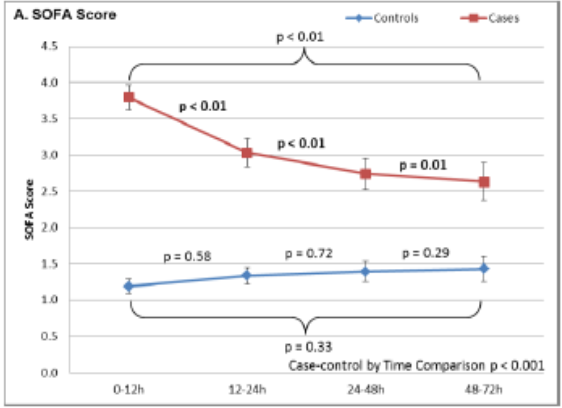
\includegraphics[scale=0.7]{Figures/SOFA_fig.png}
  \vspace{-25pt}
  \caption{\footnotesize Deterioration of the Sequential Organ Failure Assessment score (SOFA) can be detected 24-48 hours before clinical deterioration leads to ICU admission; p-values reflect pair-wise comparisons between consecutive time intervals, adjusting for patient characteristics. \cite{Yu_24970344}.}
    \label{fig:SOFA_fig}
 \vspace{-15pt}
\end{wrapfigure}

Acute respiratory failure (ARF) requiring mechanical ventilation is common in hospitalized patients, consuming a disproportionate amount of health care resources in the USA \cite{Wunsch_20639743}. Short term mechanical ventilation can be life saving, but prolonged mechanical ventilation often leads to multi-organ failure and death in a third of patients \cite{Wunsch_20639743, Ranieri_10872010}.

Most research focuses on \textit{established} respiratory failure in the ICU, while detectable clinical signs and symptoms often herald the impending respiratory decompensation much earlier \cite{Rohde_23401431}. Dr. Gong co-developed the LIPS score to identify patients at high risk for the development of Adult Respiratory Distress Syndrome (ARDS) in the emergency department \cite{Herridge_12594312}, which proved equally able to discriminate the 587 patients in the cohort who progressed to severe ARF requiring > 48 hrs of mechanical ventilation. She also demonstrated that predictive scores deteriorate as early as 24-48 hours before ICU admission  [Figure~\ref{fig:SOFA_fig}] \cite{Yu_24970344}; but such ominous signs are either not recognized or not acted upon \cite{Hillman_12415452,McQuillan_9632403}. Early interventions (e.g antibiotic therapy, diuretics and physiotherapy) and preventive measures (e.g. head elevation) would be able to stop or reverse the clinical deterioration and/or prevent progression to multiple organ failure and prolonged mechanical ventilation or at least attenuate the subsequent clinical course \cite{Naeem_16150531,Rivers_11794169,Rivers_12594312,Mitchell_20378235}. 

\begin{wraptable}{l}{6cm} 
\vspace{-25pt}
\begin{center}
\begin{tabular}{l}
\toprule
\multicolumn{1}{l}{\footnotesize Checklist interventions examples}\\
\midrule
\footnotesize \textbf{Prevent respiratory insufficiency}\\
\footnotesize \emph{Early goal directed therapy \cite{Levy_23103175}}\\
\footnotesize \emph{Adequate early antibiotics \cite{Lim_19783532}}\\
\footnotesize \textbf{Decrease mechanical ventilation} \\
\footnotesize \emph{Daily sedation break \cite{Barr_23269131}} \\ 
\footnotesize \emph{Spontaneous breathing trials \cite{Girard_18191684}}\\  
\footnotesize \textbf{Limit transfusion-related lung injury}\\
\footnotesize \emph{Restrictive transfusion strategy \cite{Hebert_9971864}}\\
\hline
\end{tabular}\\
\end{center}
\vspace{-20pt}
\caption{\footnotesize Examples of checklist interventions, references documenting effect.} \label{table:Checklist}
\vspace{-10pt}
\end{wraptable} 


\subparagraph{A pragmatic trial to predict and prevent mortality from respiratory failure in hospitalized patients.}  My mentor Dr. Gong is leading a \href{http://projectreporter.nih.gov/project_info_description.cfm?projectnumber=1UH2HL125119-01}{NHLBI-funded} multi-center cluster randomized pragmatic trial in two phases. (1) the first phase APPROVE aims to identify patients at risk by building classical logistic regression models based on electronic medical records (EMR) to Accurately Predict PROlonged Ventilation. (2) In the second phase PROOFCheck, identification of a patients at high risk triggers a decision support tool and bundled checklist interventions, proven to prevent organ failure in critically ill patients \cite{Levy_23103175,Lim_19783532,Barr_23269131,Girard_18191684,Hebert_9971864}. CITE CLINICAL TRIALS.GOV. \emph{Hypothesis:} Early implementation of a checklist of preventive measures (\ref{table:Checklist}), reduces severity of organ failure, mortality and duration of mechanical ventilationin in patients at high risk identified by APRROVE. 

\subparagraph{Electronic medical records are an eminent example of richly structured and correlated Big Data.} Exemplified by Dr. Gong's pragmatic trial, they hold enormous promise for outcomes research across a wide swath of clinical domains ranging from pediatrics to psychiatry, from maternal health to mortality from cancer \cite{Dean_19279318,Amarasingham20940649,Welch24782349,Smeeth_15602021,Dave_20819960,Man_23272239}. However, large electronic medical data sets are not just bigger in that there are more instances of the same thing, (e.g. more patients would make data analysis only easier).  Rather, there is more breadth to the data, and in the case of pragmatic trials, more heterogeneity, more subgroups, locations, or time granularity than is currently being modeled, more frequent and detailed measurements than can easily be incorporated into classical models.  This currently limits the scientific hypotheses and clinical inferences, that can be explored and evaluated. In Dr. Gong's trial in particular, we desire more fine-grained predictions to individualize prevention.  

\paragraph*{We can individualize prevention by targeting patients at risk.}
Preventive measure, for example goal targeted resuscitation, decrease respiratory failure requiring mechanical ventilation, when they are initiated early \cite{Rivers_12594312}. However, an indiscriminate approach to prevention of respiratory failure in hospitalized patients will be ineffective, because only one in 30 hospitalized adults requires mechanical ventilation. Secondly, individualizing preventive and therapeutic measures specifically based on patient characteristics will be more efficient in preventing potentially irreversible end organ damage, while also  leading to improved compliance by providers and cost effectiveness. So how can we improve and individualize prediction and prevention? 

\subsection*{Hierarchical modeling is transformative for EMR-based prediction.}

\subparagraph{Observations and outcomes in EMRs and pragmatic trials will be nested hierarchically.}
For example, in APPROVE and PROOFCheck, repetitive oxygen saturation measurements will be similar in the same patients; the closer in time they are, the higher the correlation between repeated observations. Equally, patients seen by one and same hospitalist will tend to have similar outcomes, predicted by that physician's behavior and qualities. As an example, some physicians (or services) will follow a more liberal fluid management, others will emphasize early diureses; clearly this choice will summarily affect the respiratory failure risk of specifically those patients under this physician's care. Generally, physicians in large academic medical systems like ours are organized in services, which are integrated across wards, clustered in several hospitals. Consequently, the observations in our hospitalized patient cohort, their outcomes and their propensity to respond to treatments, all are hierarchically nested; this requires more than just fitting well-known models at larger scales. 

\subparagraph*{Hierarchical models better exploit the fine-grained multilevel structures of electronic medical records} and may therefore optimally predict acute respiratory failure leading to prolonged mechanical ventilation or death in our trial cohort. Fitting our predictive regression model, we would want the regression coefficients to vary by group (e.g. by service, by medical unit, by hospital), to realistically model the multifaceted correlations seen in actual clinical practice. The number of parameters to estimate grows very quickly and so do the potential interactions. Even with very large data sets, the sample size in each subgroup will shrink rapidly; estimates using least squares or maximum likelihood will become noisy and thus often become essentially useless. One solution lies in hierarchical modeling, where we estimate hyper-parameters and hyper-hyper-parameters (Figure \ref{fig:Distrogram}), to represent how lower level parameters vary across different groupings \cite{Bafumi_Gelman_2007}. 

\begin{wrapfigure}{R}{8cm} % Example figure with text wrapping around it
 \vspace{-20pt}
 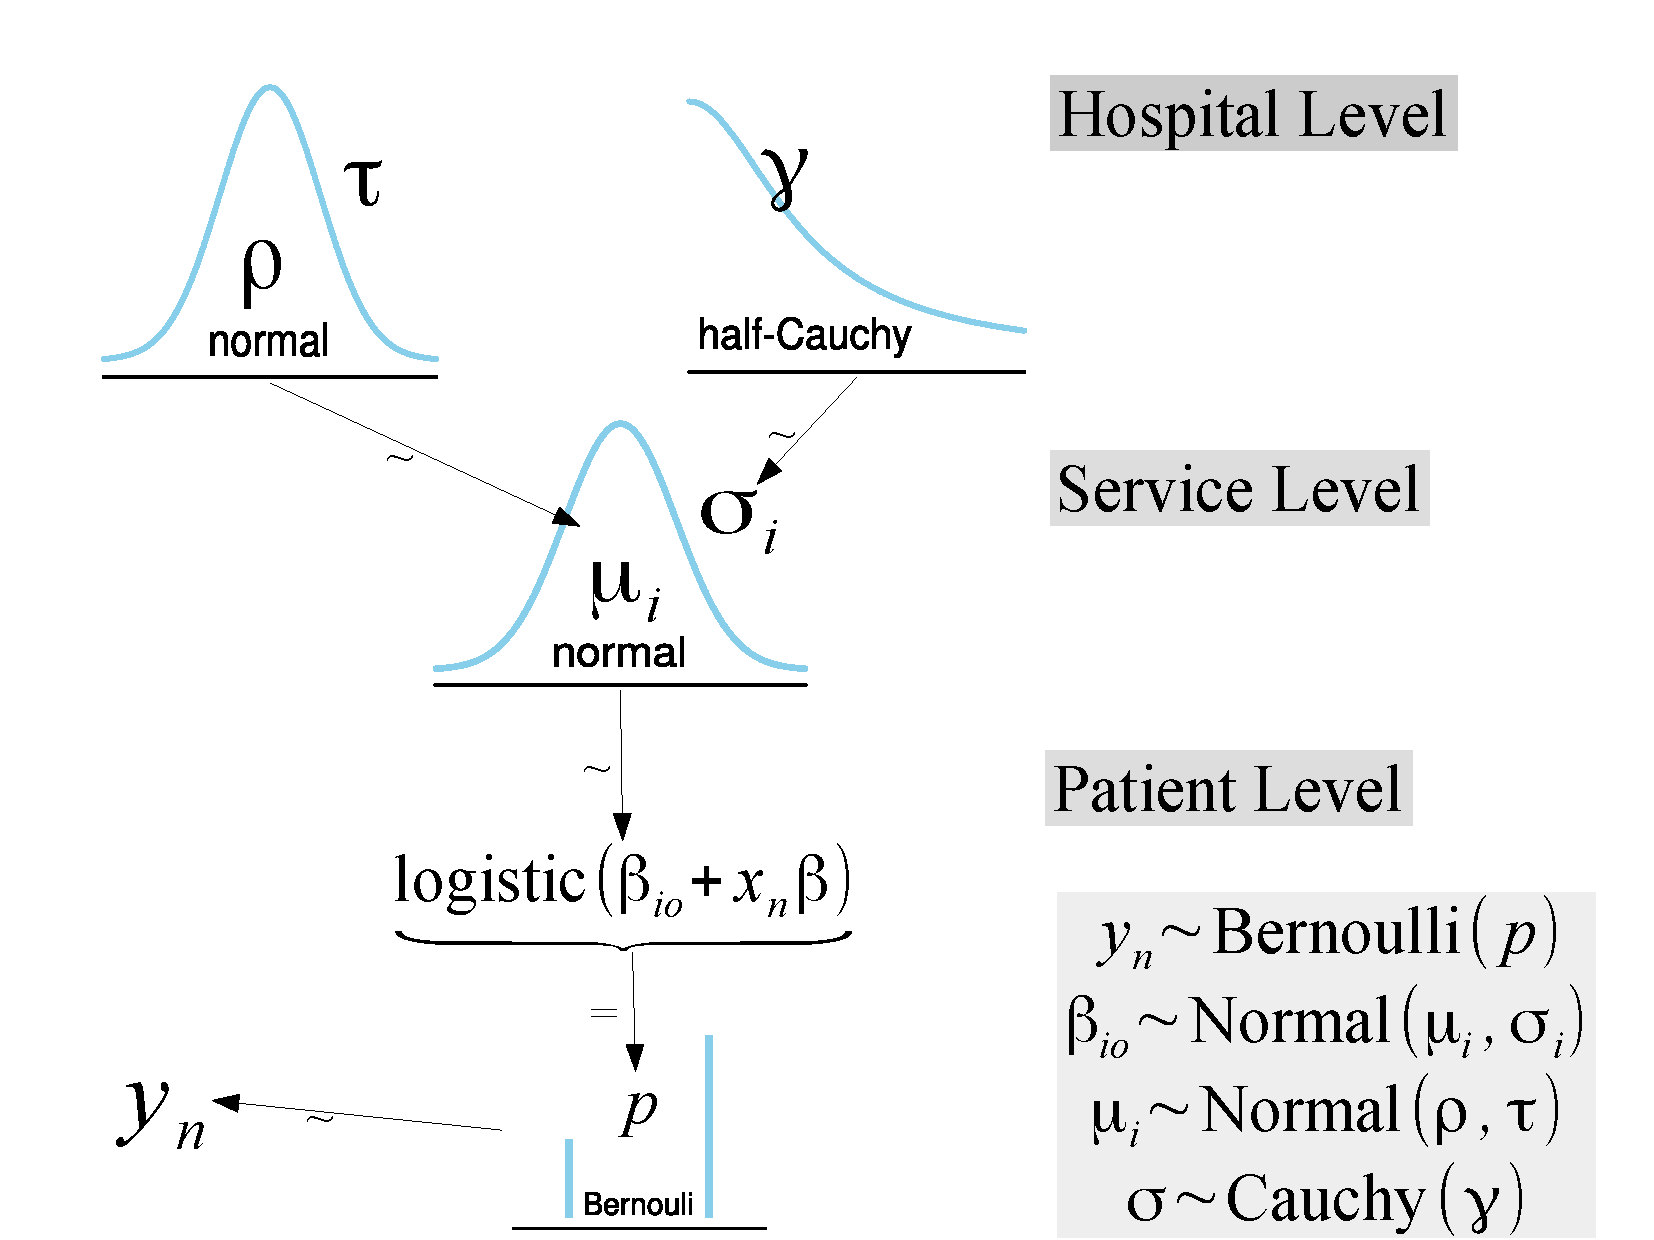
\includegraphics[scale=0.3]{Figures/Distrogram.pdf} 
  \vspace{-10pt}
 \caption{\footnotesize Distrogram to illustrated the hierarchical structure of patient trajectories. Patient level regression coefficient $\beta_0$ varies across medical services, service level mean $\mu$ and within-service variance $\sigma$ vary by hospital. }
 \vspace{-10pt}
 \label{fig:Distrogram}
\end{wrapfigure} 

\subparagraph*{Partial pooling is more efficient for prediction.}
Prediction based on "partial pooling" outperforms (a) the "No-pooling" and (b) the "Complete-pooling" approach, as can be shown mathematically or via cross-validation \cite{Gelman-Hill_2014}. Using (a) the "No-pooling" approach, we estimate the model for each specific subset of interest separately. But if we want to fully address and explore the complexity and granularity, the richness of the EMR data, this leads to far too many sub-classifications, thus too small samples in any given subgroup for useful inferences. Employing (b) "Complete pooling" or structural modeling constitutes the other extreme of the spectrum, but the implied hard constraints on the coefficients in different groups may lead to bias: we loose information, because we cannot learn from groups where we have more data. We choose the middle ground: Prediction using "partial pooling" or hierarchical modeling is especially effective for our richly organized EMR data, because the estimate of each individual parameter is simultaneously informed by data from all the other patients in our cohort, improving prediction in particular for subgroups with sparse data. \cite{Gelman_multilevel_2006}. 

\emph{We hypothesize that hierarchical modeling may better identify hospitalized patients at risk for acute respiratory failure leading to prolonged mechanical ventilation or death than the APPROVE prediction algorithm.}

\subparagraph*{Heterogeneous and incomplete clinical data may limit prediction and implementation.}
Variables with strong predictive power in our model may not be recorded in all patients or may be missing for the time window needed for prediction, limiting development of the prediction algorithm, implementation of the therapeutic interventions and the trial itself. Incomplete data are the hallmark of EMRs. In our data set we find for example that an arterial blood gas (ABG) to assess arterial oxygen tension is often unavailable for the prediction time window, because it was not requested by the physicians. To improve prediction for cases with incomplete data, we can impute the missing data using \textit{multiple imputation}. However, informative loss by non-ignorable incomplete data may bias risk prediction or may hamper the implementation of the prediction algorithm. Likelihood-based mixed effects models for incomplete data give valid estimates \textit{if and only if } the data are ignorably missing; that is, the parameters for the missing data process are distinct from those of the main model for the outcome, and the data are missing at random (MAR) \cite{Rubin_1976}. However, this is an unreasonable assumption for our electronic medical records; in our example, physicians will request ABGs based on the patients respiratory co-morbidity and clinical hypoxia symptoms. Data will not be missing at random. Instead, incomplete data will be associated with predictors and outcomes; this could lead to biased imputations.

\subparagraph*{Auxiliary data can be used to impute incomplete medical records.} Auxiliary data are additional information available in the form of variables known to be correlated with the missing data of interest \cite{Daniels24571539}. If the physician did not request an ABG, instead peripheral oxygen saturation and or oxygen therapy may be available and could be used to impute the arterial blood oxygen tension [Figure~\ref{fig:Imputation_fig}]. This approach avoids the perils associated with missing at random (MAR) assumptions, when fitting a non-ignorable missingness model \cite{Wang_20029935}.

\begin{wrapfigure}{R}{10cm} 
 \vspace{-30pt}
 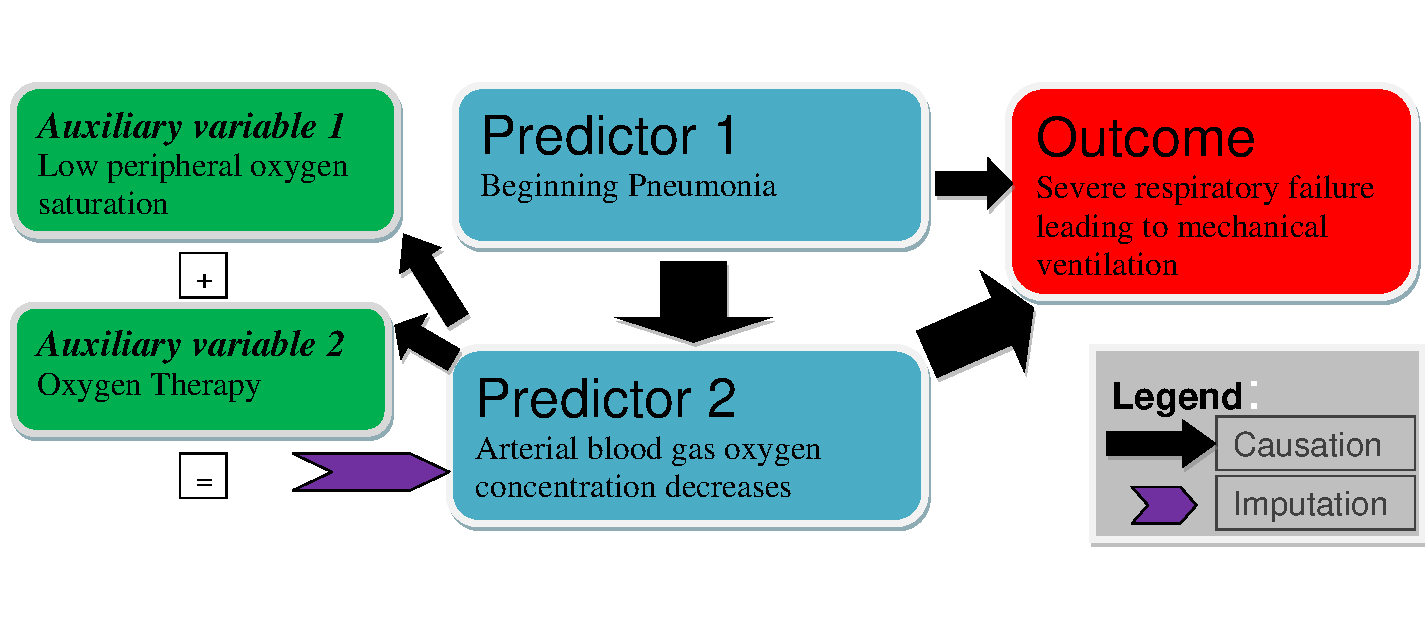
\includegraphics[scale=0.4]{Figures/Bayesian_imputation.pdf}
    \vspace{-20pt}
  \caption{\footnotesize Incomplete data can hinder outcome prediction, but we can impute incomplete data from auxilliary information. For example, pneumonia (causing to low oxygen tension), may cause respiratory failure. If arterial blood gas results are missing, we can impute the oxygen tension from oxygen therapy and/or peripheral oxygen saturation.  \cite{Hall_25389642}.}
   \vspace{-20pt}
    \label{fig:Imputation_fig}
\end{wrapfigure}

Adding auxiliary variables not included in the main model for multiple imputation, in other words using additional information that is correlated with the missing outcome is an emerging approach to help correct bias \cite{Meng_1994, Collins_11778676, Rubin_1996}, often relying on Bayesian methods for the multiple imputations approach \cite{Daniels_2008, Schafer_1997}; joint hierarchical modeling, including the use of auxiliary data to impute incomplete patient records will improve the prediction model and facilitate smoother implementation of the algorithm into the clinical trial \cite{Hall_25389642}.

\emph{We hypothesize that joint hierarchical modeling, incorporating the use of auxiliary data to impute incomplete patient records, will improve our prediction model compared to classical prediction with multiple imputation.}

\subparagraph*{Seasonal effects and institutional learning can bias risk prediction and can thwart implementation} or imperil the effectiveness of our efforts to mitigate the risks of severe respiratory failure in hospitalized patients. The composition of our hospital population, their co-morbidities and risk profiles change over time, altering which patient characteristics best predict severe adverse respiratory failure and mechanical ventilation. More importantly,  during the implementation phase of previous preventive trials we noted that providers learn, changing their behavior as a result of trial participation. As trials progressed providers implemented previously underutilized interventions more frequently even before they were prompted. We term this effect institutional learning. On the other hand, the transition of junior and senior providers through their training and to other institutions and new personnel joining the staff, may led to lessons learned being forgotten again. Last but not least, respiratory disease is affected by seasonal and secular effects; influenza prevalence for example is seasonal and characterized by major and minor epidemics. Seasons and epidemics will affect the predictive power of any model and hence also alter the risk profile of our patients over time. Institutional culture and individual provider behavior change in response to trials and quality improvements interventions; patient populations change over time. 

Respiratory patients are plagued by seasonal deterioration. These temporal, seasonal and secular effects will alter the predictors of risk in our model and affect its implementation. We will therefore include institutional learning, seasonal effects and continuously update our model with new patient data to account for said changes in the risk profile. The integration EMR-triggered prediction and prevention with  institutional learning, secular and seasonal effects as well as data imputations from auxiliary data within one coherent (Bayesian) model is certainly novel, but how can it be implemented in one coherent model? 
\vspace{30pt}

\section*{B. Innovation}

\begin{wrapfigure}{l}{4.5cm} % Example figure with text wrapping around it
 \vspace{-10pt}
 \href{http://en.wikipedia.org/wiki/Bayes'_theorem}{ 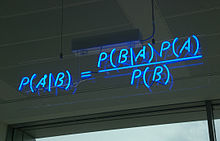
\includegraphics[scale=0.6]{Figures/BayesTheorem.jpg}}
  \vspace{-20pt}
 \caption{\footnotesize Bayes Theorem: The posterior probability $P(A|B)$ is the prior probability $P(A)$ updated with the  likelihood $P(A)$}
 \vspace{-20pt}
 \label{fig:BayesTheorem}
\end{wrapfigure}

\subparagraph*{Bayesian hierarchical modeling is groundbreaking in EMR-based prediction}, and particularly suited for joint hierarchical modeling. With their inherent flexibility and robustness \cite{Carlin_1349763,Sutton_2012}, Bayesian hierarchical models may outperform classical models for EMR-based prediction owing to the integration of additional information through "partial pooling" \cite{Gelman_red_2009} and the imputation of incomplete records from auxiliary data. Thomas Bayes formulated the Bayes theorem already in 1763 as an alternative statistical model \cite{Thomas_Bayes}. With a well developed theory, Bayesian methods are only novel in so far as they were rarely used in medical research until computers and Markov Chain Monte Carlo algorithms became widely available in the 1990s, leading to an expansion of applied Bayesian work \cite{Ashby_16947924,Spiegelhalter_11134920}, more recently also EMR-based prediction \cite{Himes_19261943,Ryynaenen_23496851,Wu_20473190} and Big Data \cite{Yoo_24987556}, but we are unaware of any Bayesian hierarchical prediction model based on large EMRs. Past constraints in computational implementation have largely been overcome, except for very large dense data sets like EMRs. 

\subparagraph*{A brief introduction to Bayesian inference and its computational implementation.}

According to Bayes' Theorem, shown in Figure \ref{fig:BayesTheorem}, prior information $P(A)$ is combined with new data $P(B)$, (known as the likelihood) to yield an \textit{updated} estimate for the probability of a hypothesis $P(A)$ given the data $P(B)$, called the posterior distribution $P(A|B)$ \cite{Kruschke_Book_2014}. The Bayesian approach is hence analogous to clinical decision-making \cite{Spiegelhalter_11134920}. Physicians continuously update their preliminary diagnosis as new information comes in. Prior belief $P(A)$ in a diagnosis may be weakened by new laboratory information $P(B)$, leading to an alternative, updated diagnosis given the lab data $P(A|B)$ \cite{Kruschke_22774788}. 

\subparagraph*{\text{Posterior probability} $\propto$ \text{Likelihood} $\times$ \text{Prior probability}.}

Bayesian inference for multi-layered (hierarchical) models can often not be derived analytically; instead we calculate numerical approximations of the multi-dimensional integrals to obtain the posterior distributions of the parameters of interest. In technical terms, Markov Chain Monte Carlo (MCMC) based Bayesian inference methods sample from a posterior probability distribution after building a Markov chain. In lay terms, MCMC simulation replaces intractable analytical integration with empirical summaries of samples from the posterior distribution \cite{Abrams_9483729}: \textit{Instead of analyzing the odds, we simulate throwing the dice repeatedly.} But MCMC simulations can be slow to converge for large EMRs.

\begin{wrapfigure}{R}{0pt}
 \vspace{-70pt}
 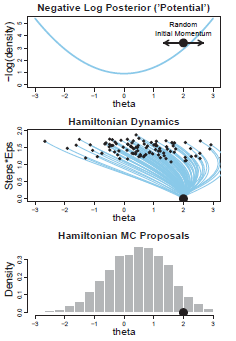
\includegraphics[scale=1]{Figures/Hamiltonian.png}
  \vspace{-30pt}
  \caption{\footnotesize Hamiltonian MCMC uses momentum to optimize the next proposal. The higher momentum of the current position (black dot) is indicated in the top panel. The middle panel illustrates how random samples are drawn to the mode of the posterior distribution (lower panel) leading to faster convergence and higher effective sample size. Fig 14.1 in Kruschke \cite{Kruschke_Book_2014}.}
    \label{fig:Hamiltonian}
 \vspace{- 1 pt}
\end{wrapfigure}

\subparagraph{Pushing the envelope of Bayesian inference for EMR-based prediction}
We will implement the Bayesian model in parallel in the ultra-fast probabilistic programming language software Stan developed by my co-mentor Dr. Gelman \cite{Stan_Software_2014} and named after Stanislaw
Ulam, who invented the Monte Carlo method with Metropolis \cite{StanislawUlam_1949}. Stan's Hamiltonian Monte Carlo algorithms \cite{Stan_Software_2014} and clever statistical formulation or manipulation push the boundaries of computability \cite{Gelman-Hill_2014}. For example non-centered parameterization allows to sample in the standardized normal space, enhancing the effective sample size in Stan and will take full advantage of the faster convergence to overcome computational limitations of Bayesian hierarchical models also for very large EMR data sets \cite{Gelman-Hill_2014}. For example non-centered parameterization allows to sample in the standardized normal space and will take full advantage of the faster convergence and higher effective sample size of Stan and overcome computational limitations of Bayesian hierarchical models for Big Data \cite{Gelman-Hill_2014}. Stan  is based on Hamiltonian Monte Carlo (HMC) \cite{Gelman-Hill_2014}, a Marcov chain Monte Carlo (MCMC) algorithm, which avoids the sensitivity to correlated parameters that plague many MCMC methods by introducing auxiliary momentum variables \cite{Homan_Gelman_NUTS_2014} as illustrated in Figure~\ref{fig:Hamiltonian}. HMC is dependent  on tuning the reciprocal relationship of the crucial parameters step size and desired number of steps. If the latter is too large, efficiency is low, if to small we see undesirable random walk behavior. To overcome this, Dr. Gelman's team developed and implemented the No-U-Turn Sampler (NUTS), a recursive algorithm to automate and optimize tuning the HMC \cite{Homan_Gelman_NUTS_2014}.
  
\subsection*{Analyzing and advancing implementation is decisive for outcome improvement and research.}
Imperfect fidelity (poor provider compliance) is a major concern also in our PROOFCheck trial, just as non-compliance is a major obstacle to the effective delivery of health care and improved outcomes in general
\cite{Duncan_16710766}. The targeted interventions triggered by our EMR-prediction algorithm will only prevent respiratory failure if our physicians and nurses actually implement them. Improving fidelity of health care providers with evidence based interventions continues to be a challenge and is under-researched \cite{Davis_7650822} and little is known on how to reproduce multi-faceted interventions (specially directed toward providers) to improve clinical outcomes \cite{Campbell_10987780}. As long as we do not understand what drives provider fidelity and patient compliance with the preventive measures proposed to our providers for their high risk patients  \cite{Mittman_15172904}, we ignore the best means to translate widely accepted interventions and new findings of outcomes research into practice \cite{Glasgow_17150029}. We need to understand better what patient and/or provider characteristics hinder compliance with the triggered preventive checklist interventions to ensure care is in accordance with accepted evidence based best practices.

\subparagraph*{We use a pragmatic trial to investigate provider fidelity.} Pragmatic trials like Dr. Gong's may result in valid more estimates of effectiveness for more realistic health care scenarios \cite{Selby_22824225,Tosh_21842618}; we will use her pragmatic trial data to investigate incomplete fidelity, heterogeneity and difficulty in clinical implementation. An example with problematic fidelity relevant for PROOFCheck is blood product management; transfusions increase the risk of acute severe respiratory failure with mechanical ventilation \cite{Kenz_24892308};  recent research led to consensus that overzealous and empiric transfusion of blood products leads to worse outcomes \cite{Hebert_9971864}, acknowledging that untreated anemia also predicts poor outcome \cite{Ranucci_22698773}; guidelines reflect this for over a decade \cite{ASA_25545654}, but implementation of rational transfusion blood product management is still sketchy and very heterogeneous across the nation \cite{Likosky_20488928}; not least because their complicated algorithms can be difficult to follow. Weiss et al. demonstrated that direct prompting for best practices improves provider compliance in the ICU and outcomes such as duration of mechanical ventilation or length of stay \cite{Weiss_21616996}. We hypothesize that fidelity will be associated with certain provider and patient characteristics; their investigation will allow more focused re-education efforts and adaptation of the checklist implementation. 


\subsection*{Summary of the impact}
Acute respiratory failure in hospitalized patients leading to prolonged mechanical ventilation with the inherent mortality and morbidity constitutes a serious health care challenge. We will tackle this by combining innovative approaches to data imputation with sophisticated hierarchical prediction models to form a near real-time EMR-based clinical decision tool with practical utility in critical care. We use the opportunity to investigate poor provider fidelity a serious and under-researched barrier to outcomes research the implementation of evidenced-based care. Our findings will have implications beyond our trial for any clinical research, indeed for the implementation of evidence-based-medicine at large. Changes in reimbursement give providers a stake in patient outcomes and led to a keen interest in the prediction and prevention of adverse event in hospitalized patients. This project advances hierarchical Bayesian models to implement this paradigm shift in very large EMRs, triggering personalized interventions that deliver outcome improvements. This is novel and has not been attempted to our knowledge.

But our impact goes beyond improving morbidity and mortality from respiratory disease in hospitalized patients through improved prediction and prevention, beyond investigating drivers of poor provider compliance. We will develop new methods to impute incomplete electronic medical records from auxiliary data and pioneer Bayesian hierarchical prediction models for large EMR data. Our proposal is unique and novel in its integration of cutting edge methods from clinical, statistical and computer science to fully realize the promise of Big Data in perioperative medicine.


\section*{C. Approach}
My research project will be closely aligned with my mentor's NIH-funded pragmatic two phase trial. Aim 1 will utilize the processed data of APPROVE to improve the prediction model and Aim 2 will use the data from the implementation of PROOFCheck to investigate fidelity of the providers with the EMR-triggered interventions.

\subsubsection*{Aim 1: To improve early prediction of prolonged respiratory failure and death in hospitalized patients.}

\begin{flushleft}
\textit{Hypothesis: The Integration of multi-level (hierarchical) Bayesian modeling and data imputation will improve prediction of severe respiratory failure in hospitalized patients compared to the classical statistical approach.}
\end{flushleft}

\subparagraph*{For specific aim 1a,} we will build a pragmatic EMR-based hierarchical Bayesian model to predict a composite outcome [mechanical ventilation prolonged beyond 48 hours or death] in hospitalized adult and compare our Bayesian approach with the existing frequentist algorithm used by Dr. Gong in her pragmatic trial.

\subparagraph*{Population:}
We will include all adults patients, admitted to the Montefiore Medical Center during the study period, excluding only those who are chronically ventilated at home or who have Do not resuscitate orders at the time of hospital admission (Table 1: Inpatient population at Montefiore Medical Center.) As part of APPROVE, the pragmatic trial by Dr. Gong described in detail under Significance, two 3-month, prospective, observational cohort studies are underway at several Albert Einstein College of medicine and Mayo Clinic Rochester and Florida sites; we will build our Bayesian hierarchical model based solely on Einstein patients: Patients from the first three months will serve as the fitting cohort, while the 2nd cohort will serve as the validation and test set.  

\subparagraph*{Predictors:}
Many independent variables are candidates for potential inclusion into our Bayesian hierarchical model. From the multicenter LIPS study, clinical factors most closely associated with prolonged mechanical ventilation have already been identified \cite{Herridge_12594312}. We will consider these and additional time-invariant and time-variant demographic and clinical data. Examples for demographics are gender, age, medical service or ward, examples for physiological and clinical predictors are heart rate, blood pressure or lab tests, respectively. Certain predictors will require summary aggregations and (logarithmic) transformations to induce variance stability.

\subparagraph*{Outcomes:}
Our primary dichotomous outcome will be acute respiratory failure requiring mechanical ventilation longer than 48 hours. Outcomes are specified as positive for (a) mechanical ventilation lasting longer than 48 hours or (b) mechanical ventilation lasts less than 48 hours, but the patient died within 96 hours of the calculated score. Patients that are not on prolonged ventilation within 96 hours or discharged alive from the hospital will be considered negative.


\subsubsection*{Bayesian hierarchical modeling to reflect the nested structure of health care}   
We will build a Bayesian hierarchical multivariate logistic regression model of time-invariant and time-variant demographic, clinical and administrative variables. Our Bayesian hierarchical modeling will represent the multi-level nested structure of current health care, with levels for medical or surgical service the patient is under, the floor or ward where the patient is cared for, the institution the patient is admitted to. We will also consider other random effects for example for co-morbidity and other time-invariant patient specific descriptors. We illustrate this nested structure in a simple logistic model with hierarchical levels for patient, service and hospital. 

\begin{wrapfigure}{l}{.5\textwidth}
\vspace{-20pt}
 \begin{equation} \label{eq:patientlevel}
 Y \sim Binom (\alpha, n); \alpha = inv\_log (\beta_{0} +\beta_{1} * PaO_2)
 \end{equation}
\vspace{-25pt}
\end{wrapfigure}

\subparagraph*{Patient level (\ref{eq:patientlevel})}
On the left, we model at the patient level, the probability $alpha$ that a patient will develop the dichotomous event $Y$, acute respiratory failure requiring mechanical ventilation, using arterial oxygen tension $PaO_{2}$ as a predictor in a simple logistic regression model. However, patients are typically assigned to hospital services. Pulmonary service patients may have a lower baseline $PaO_2$, while surgical patients tend to have normal lung function. 

\begin{wrapfigure}{l}{.5\textwidth}
\vspace{-10pt}
\begin{equation} \label{eq:servicelevel}
 \beta_{0} \sim Normal (\gamma_0 , \tau_{\beta_0}); \beta_{1} \sim Normal (\gamma_1, \tau_{\beta_1})
\end{equation}
\vspace{-25pt}
\end{wrapfigure}

\subparagraph*{Service level (\ref{eq:servicelevel})}
On the left we develop our hierarchical model to allow different intercepts $\beta_{0}$ representing the average $PaO_2$ of patients in the various medical and surgical services estimating different service level mean intercepts $\gamma_0$. Under a medical service, smaller changes in $PaO_2$ may be indicative of respiratory deterioration compared to a surgical service, where larger drop in arterial oxygen tension predicts outcome. We may allow the regression coefficient for the slope $\beta_{1}$ to vary around different mean slopes $\gamma_1$ at the service level. 

\begin{wrapfigure}{l}{.5\textwidth}
\vspace{-10pt}
\begin{equation} \label{eq:hosptiallevel}
\gamma_0 \sim Normal (\delta_{tau_{0}}, \zeta); \tau_{\beta_1} \sim Normal(\delta_{tau_{1}}, \kappa) 
\end{equation}
\vspace{-25pt}
\end{wrapfigure}

\subparagraph*{Hospital level (\ref{eq:hosptiallevel})}
Some hospitals may cater to an economically disadvantages population, which is sicker on average. To reflect this, we may  model the mean intercept $\gamma_0$ for the services hierarchically at the hospital level. Some hospitals are organized such that patients differ very much between services, other hospitals may have a more homogeneous patient distribution; this \textit{variation} $\tau_{\beta_1}$ of the mean slope $\gamma_1$ within services at a given hospital can also be modeled to capture the variability of the predictive effect of lower $PaO_2$.
 
\subparagraph*{In APPROVE, the compared frequentist prediction model will be build by Dr. Gong's statistical team} employing the published LIPS score \cite{Herridge_12594312} to identify hospitalized patients at risk for prolonged mechanical ventilation and death. The score at the selected start time will be used to determine the best cutoff score to identify the patients with the highest risk of developing prolonged mechanical ventilation.

\subparagraph*{Data Acquisition}
Data will be abstracted from a clinical data warehouse(see Environment and Resources). A multi-prong approach for capturing complete, longitudinal data in real-time, near real-time, or asynchronously from the EMR replica will be used. When possible, and where collection of additional complementary information is warranted, we will use the Retrieve Form for Data Capture IS THIS THE CORRECT REFERENCE?\cite{Rothenhaeusler_2005},an IHE30 IS THIS THE CORRECT REFERENCE? \cite{Rotte_15809512} standard for gathering new data within a user's current application environment (EMR in this case) to meet the requirements of an external system. Secured electronic data capture tools provided by the Montefiore Enterprise Clinical Research Management System will be used to streamline, quality control, normalize, and manage data collection and data entry efforts. A fully de-identified, study specific database of all study variables will be compiled for model development and validation. When subsequently patient data from additional regional medical centers are incorporated, site identifier variables will be obfuscated to blind investigators.

\subparagraph*{Model checking}
We will look at auto-correlation, trace-plots and calculate the Gelman and Rubin's MCMC Convergence Diagnostic $ \hat{R}$ to evaluate the the convergence of our Markov chain Monte Carlo (MCMC) simulations using \href{http://andrewgelman.com/2015/03/02/introducing-shinystan/}{shinyStan}, the interactive visual application to graphically explore hierarchical models, we developed \cite{shinystan-software:2015}. Others reviewed shinyStan's installation and utility on \href{https://www.youtube.com/watch?v=X31xqNHcvQs}{YouTube}. In evaluating our Bayesian model's predictive performance, exploratory graphical \cite{Gelman2004posteriorpredictivechecks} and confirmatory formal posterior predictive assessment using discrepancies \cite{GelmanMengStern1996} will complement each other to compare the patient test set to simulated replications from our fitted hierarchical Bayesian model. As a simple example, for each draw of the estimated parameter $\theta$ from the posterior $p(\theta|y)$ we simulate data $y^{rep}$ from the posterior predictive distribution $ p(y^{rep}|y) $. Using the simulations of $y^{rep}$ we can make various graphical displays comparing our observed data to the replications:

\begin{wrapfigure}{l}{.35\textwidth}
\vspace{-11pt}
\begin{equation} \label{eq:predictivecheck}
 p(y^{rep}|y)  = \int \! p(y^{rep}|\theta) p(\theta|y) \, \mathrm{d}\theta 
\end{equation}
\vspace{-20pt}
\end{wrapfigure}

If our model is a good fit, then data generated by the model using the estimated parameters should have a distribution similar to the original data we observed. We illustrate this idea behind posterior predictive checking \cite{Gelman_predictive_2000} in Figure~\ref{fig:posteriorpredictivecheck}, generated in our software package shinyStan \cite{shinystan-software:2015}:

\begin{wrapfigure}{r}{.3\textwidth} 
 \vspace{-15pt}
 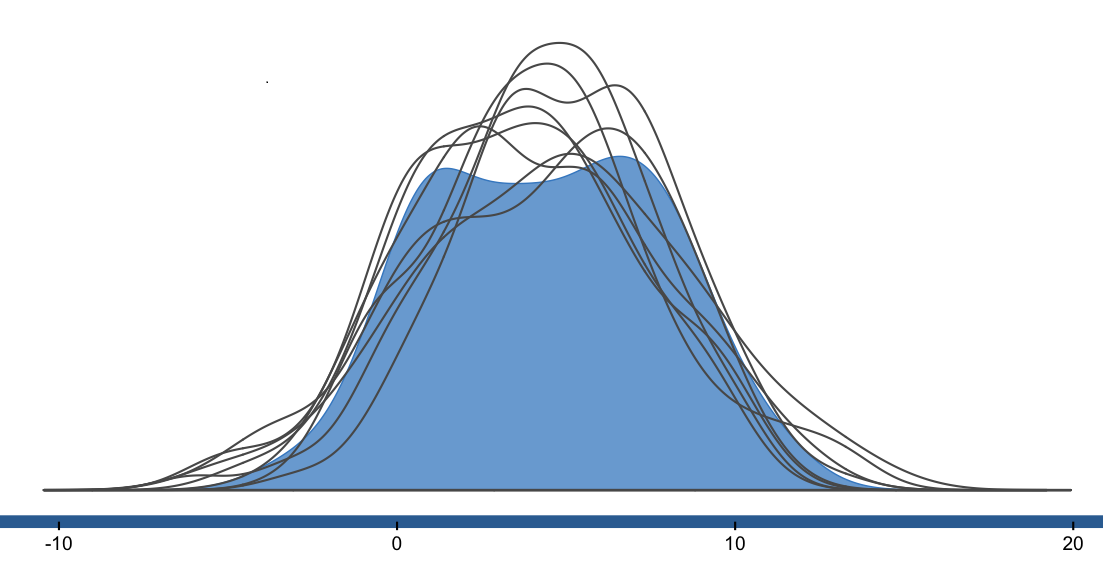
\includegraphics[scale=0.2]{Figures/posteriorpredictivecheck.png} 
  \caption{\footnotesize Exploratory posterior predictive checking using our software shinyStan \cite{shinystan-software:2015}: Visual comparison of the distribution of observed data (shaded in blue) to the distributions of the data simulated (thin lines) suggest a reasonable model fit.}
  \label{fig:posteriorpredictivecheck}
\end{wrapfigure}

As a more sophisticated approach we will graphically contrast the vector test statistics $T(y)$ versus replicated data $T(y^{rep})$ to detect a potential misfit of model to data \cite{Gelman2004posteriorpredictivechecks,Buja1999inference} Analogously, we will use predictive validation to adjust for overfitting of our model and perform a sensitivity analysis of our priors on key model parameteters \cite{Gelman-Hill_2014,Gelman_predictive_2000}.



\subparagraph*{Model comparison}
We will assess the plausibility of our posited hierarchical model and its assumptions \cite{Gelman_predictive_2000,GelmanMengStern1996} and will compare it to the alternative classical model by Dr. Gong (based on a non-nested much simpler model \cite{Herridge_12594312}). As a simple approach, we will perform a nonparametric comparison of areas under the curve (AUC) of the correlated receiver operating characteristics (ROC) curves \cite{DeLong_3203132} to assess their respective predictive performance \cite{Newcombe_22890972,Wu_20473190}, in other words to investigate if the hierarchical modeling improves prediction of acute severe respiratory failure over the simpler classical model used by Dr. Gong. We will compare the models based on a different test set from the same population, to avoid biasing the comparison in favor of our more complicated, (possibly overfitted) hierarchical model. Cross-validation is widely used to compare statistical models for estimating out-of-sample prediction error \cite{Vehtari_12396570}. However, in our case, we operate on the limits of computability and repeatedly fitting our Bayesian hierarchical model to leave-one-out samples, could be computationally too expensive \cite{Gelman_Aki_2014predictive}. Besides, for multi-level data, leaving partitioning the data for cross-validation should probably consider the hierarchical structure itself; indeed, cross-validation may not always be a sensitive instrument for model comparison \cite{wang_predictive_2014}. Hence, we will also explore the predictive information of our hierarchical model using posterior predicitve simulations and realized discrepancies \cite{Gelman_Aki_2014predictive,Gelman_predictive_2000,GelmanMengStern1996}. In parallel sampling \cite{Congdon_modelcomparison_2005}, we will compare our Bayesian Model to the classical simpler algorithms using the minimum $\chi^{2}$ discrepancy, essentially equivalent to the classical
goodness-of-fit test statistic \cite{GelmanMengStern1996}. For additional validation and as a safeguard against over-fitting, we will train our model with patient data from other participating institutions (Mayo Clinic Rochester and Florida) and test if our model outperforms the classical prediction models even in other ecological settings, both if the classical frequentist model is based on data from all institutions or the test institution (say Mayo Clinic Rochester) alone. 

\begin{wrapfigure}{l}{.35\textwidth} 
 \vspace{-10pt}
 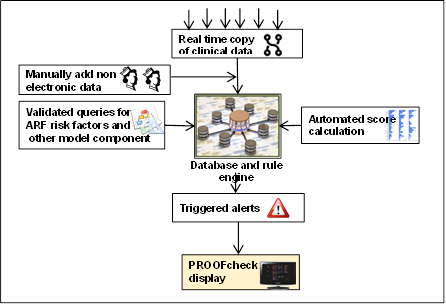
\includegraphics[scale=0.55]{Figures/Alert_trigger_fig.png} 
  \caption{\footnotesize Illustration of the implementation algorithm. A real time EMR copy is scanned for risk factors for acute respiratory failure. Providers are promoted to initiate prevention specifically for their patients identified as at risk.}
   \vspace{-20pt}
  \label{fig:implementation}
\end{wrapfigure} 

\subparagraph*{Technical approach}
Boolean combinations of data matching and natural language processing of the prediction algorithms will be used to scan a real time copy of the hospital's clinical and administrative data including demographic, monitoring, pharmacy, laboratory, and physician notes for risk factors and physiological abnormality. Figure~\ref{fig:implementation} illustrates the implementation algorithm. The rule engine (implemented in Java) will send out the alert to providers.
We will integrate Bayesian patient triage into the infrastructure established during PROOFCheck, Dr. Gong's pragmatic trial, if we can show that our Bayesian prediction algorithm is superior to the existing algorithm. Based on our analysis for aim 2, compliance information will be reviewed for various items during the course of study so that sites could be targeted for re-education.

\subsubsection*{Imputing incomplete EMR-data using auxiliary data}

Missing data are a characteristic limitation of large electronic medical records and may bias our prediction model \cite{Dean_19279318}. Electronically medical records measurements not updated 24 hours earlier than the selected start time will be considered missing;  as an illustrative example, we formulated a simplistic model illustrated in [Figure~\ref{fig:Imputation_fig}]. We combine the prediction of the dichotomous compound outcome $Y$, (defined as acute respiratory failure leading to mechanical ventilation and death) using latent arterial oxygen tension $\Omega$ in a logistic regression model in Equation \ref{eq:Impute1} and \ref{eq:Impute2}: 
\begin{wrapfigure}{l}{.3\textwidth}
   \vspace{-25pt}
\begin{align} \label{eq:Impute1}
Y \sim Binom(\mu, n)\\ 
\mu = inv\_log(\beta_{0} + \beta_{1} * \Omega)\label{eq:Impute2}
\end{align}
   \vspace{-25pt}
\end{wrapfigure}

We may have the $PaO_{2}$ from an arterial blood gas (ABG) or not. Nota bene, ABGs will certainly not be missing at random, but contingent on the $PaO_2$ value and respiratory outcome $Y$. If the $PaO_{2}$ from the ABG is observed, we will use it to predict the outcome $Y$. If no ABG was obtained, we impute the latent oxygen tension $\Omega$ with a regression model from the auxiliary data  $O_{2}$ Saturation and $O_{2}$ therapy:
 
\begin{wrapfigure}{l}{.6\textwidth}
   \vspace{-25pt}
\begin{align}\label{eq:Impute3}
\Omega =  I(observed = true) * PaO_{2}   +   I(observed = false) * \delta  \\ 
\delta \sim Normal(\theta, \tau); 
\theta = \gamma_{0} + \gamma_{1}* O_{2} Sat + \gamma_{2} * O_{2} Therapy \label{eq:Impute4}
\end{align}
   \vspace{-25pt}
\end{wrapfigure}

Our imputation approach exploits the temporal relationship between variables in the longitudinal electronic medical records \cite{Welch24782349}. We will identify the auxiliary measure properties, ceiling and floor and potential threshold effects effects, test the imputations against manually verified data and published algorithms and compare them to the simple and multiple imputation strategies planned for Dr. Gong's pragmatic trial \cite{Huntington_16311133,Sloan_15027501}.  We will perform posterior cross validation checks to investigate the appropriateness of our assumptions and incomplete data model \cite{Gelman1998notasked}.

\subsubsection*{Aim 2: To model temporality (institutional learning, seasons) and investigate provider compliance.}
To most closely reflect the realistic situation of actual academic and community medical delivery settings, we need to take temporal and seasonal changes changes into account. To focus education efforts and improve implementation of preventive or therapeutic measures, we will investigate predictors of provider behavior. 

\paragraph*{For specific Aim 2a,} to reflect changing risk profiles over time, we will adjust our Bayesian model to update continuously with new incoming patients and adapt our model to include temporal effects, like institutional learning, seasonal or endemic phenomena. Seasonal changes could for example be modeled by adding another level above the hospital level modeled in Equation \ref{eq:hosptiallevel} to our patient-service-hospital hierarchy illustrated in Figure \ref{fig:Distrogram}:

\begin{wrapfigure}{r}{.25\textwidth}
   \vspace{-20pt}
\begin{align}\label{eq:SeasonLevel}
\delta_{tau_{0}} \sim Normal(\phi, \psi) 
\end{align}
   \vspace{-30pt}
\end{wrapfigure}

Equation \ref{eq:SeasonLevel} would thus allow the hospital level mean to vary over time to reflect increases in the severity and prevalence of chronic obstructive pulmonary disease in the winter or to smooth over differences in annual flu prevalence. 
  
\paragraph*{For specific Aim 2b,} we will investigate provider compliance with the individual components of the checklist. During the second phase (PROOFCheck) of Dr. Gong's pragmatic trial, providers of a patient identified as high risk by the frequentist prediction algorithm will be prompted electronically to implement concrete preventive and corrective measures from a list of widely accepted interventions. During roll-out, providers receive targeted education on prevention and best practice. During PROOFCheck implementation, physician are notified by pager and/or electronic clinical interface; an interactive notification algorithm will suggest patient specific interventions from the checklist to the clinicians. 

\paragraph*{Prediction of adverse events is useful only if followed by effective preventive action. } We will use data from PROOFCheck, the second phase of Dr. Gong's pragmatic trial to analyze provider compliance (fidelity) with the proposed interventions. In particular, we will investigate which provider and patient characteristics predict compliance with which components of the intervention checklist. My project will be to investigate patient and provider characteristics as drivers of poor provider compliance in PROOFCheck, Dr. Gong's pragmatic trial. This will inform the ongoing PROOFCheck trial implementation, in which I will actively participate. Hence my concurrent results will immediately refocus our retraining efforts during PROOFCheck. Finally we will explore the individualization of preventive interventions using EMR-context. 

\begin{wraptable}{r}{4.7cm} 
 \vspace{-15pt}
 \begin{center}
    \begin{tabular}{l l r}
\toprule
 \multicolumn{1}{c} {\footnotesize Hospital} & {\footnotesize Beds} &{\footnotesize Vent\textsuperscript{a}}\\
  \midrule
  \footnotesize Montefiore & 620 & 815\\
  \footnotesize Weiler & 396 & xx\\
  \footnotesize Wakefield & 369 & xx\\
  \footnotesize Mayo Clinic & xxx & 440\\
  \footnotesize BIDMC & 646 & 2,204 \\
 \footnotesize \emph{Total} & xxx & xx \\
\hline
 \vspace{-20pt}
    \end{tabular}\\
 \caption{\footnotesize PROOFCheck hospital population (\textsuperscript{a}{patients ventilated})} \label{table:populations}
 \end{center}
  \vspace{-25pt}
\end{wraptable}

\paragraph*{Population:} 
Only data from those hospitalized adults identified by the classical algorithm developed during APPROVE as high risk for developing severe acute respiratory failure with prolonged mechanical ventilation and intubated patients will be included during this second phase (PROOFCheck). We will include all data from all participating centers. Hospital beds and annual numbers of ventilated patients for each hospital are presented in Table \ref{table:populations}. Patients chronically ventilated at home or who have DNR, will be excluded. PROOFCheck will limit recruitment to wards found to have higher prevalence of severe adverse respiratory events during the first phase of Dr. Gong's trial (APPROVE). 

\subparagraph*{Exposures and predictors:}
Provider and/or patient characteristics could be drivers of poor fidelity and adherence. We will consider time-invariant and time-variant provider and patient demographic and clinical data. We hypothesize two example of provider and patient demographics as predictors fidelity: (1) junior residents may be less comfortable with stricter blood transfusion triggers compared to seasoned physician assistant,; (2) providers fidelity with evidence based treatment recommendations may be contingent on patient gender, in particular in heart failure \cite{Cook_25714825}, likely an important predictor of acute respiratory failure in APPROVE. Time-variant patient characteristics (e.g. lab values) could determine provider fidelity; for example borderline blood hemoglobin concentration will likely influence compliance with blood transfusion recommendations issued during PROOFCheck. 

\subparagraph*{Outcomes: The unit of analysis is the triggered intervention.}
The primary outcome will be provider compliance, a dichotomous event, defined as positive if the provider ordered the prompted preventive intervention. In order to measure and demonstrate compliance with the checklist, near real time (same day) transaction logs and evidence for compliance will be recorded through electronically.

\subparagraph*{Study design and model building}
This is a prospective observational cohort study to investigate sustained provider fidelity with EMR-triggered preventive interventions in PROOFCheck, Dr. Gong's pragmatic multicenter trial. We will build a Bayesian hierarchical multivariate logistic regression model of time-invariant and time-variant demographic, clinical  and administrative variables, with levels for service, ward and institution, analogously to aim 1; the hierarchical structure is to reflect certain biases and attitudes ingrained in certain medical or surgical specialties or hospital wards, which may lead to different associations between provider and patient characteristics and provider fidelity with treatment prompts, for example service-specific reluctance to use triggers to minimize blood cell transfusion \cite{Goodnough_23706801}. 


\subparagraph*{Sustained implementation of our Bayesian algorithm with extension to other regional institutions.} Beyond, PROOFCheck, we will continue to trigger individualized patient interventions to the providers in the Einstein system, if the EMR triggered intervention checklist proves to be effective. We will integrated our Bayesian model into the PROOFCheck infrastructure to sustain the outcome improvements, if our Bayesian imputation and prediction outperforms the classical algorithms.

\subparagraph*{Data collection, institutional review and data safety and monitoring board:} we will collect patient and provider characterizes and record provider compliance with EMR-triggered alerts in real time prospectively to investigate predictors of provider behavior in generalized linear models as described in more detail in aim 1. As detailed under aim 1, he IRB approved both APPROVE and PRROFcheck, including the data collection for provider compliance. We will apply for minor amendments of this IRB approval.
 
\subsubsection*{Limitations and feasibility of our research plan }

\begin{figure}[h]
 \vspace{-20pt}
 \centering
   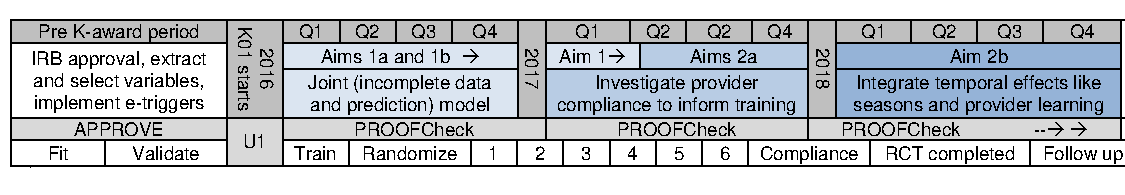
\includegraphics[scale=1]{Figures/Timeline.pdf}  
 \vspace{-30pt}
 \caption*{\footnotesize \textbf{Timeline:} My research plan is well aligned throughout the award period, with the time axis on top, trainee project in the second row and the mentors U1 grant timeline below. }
  \vspace{-10pt}
  \label{fig:Timeline}
 \end{figure}
 
The timelines of my research plan and my mentors U1 project are well aligned as illustrated in the Timeline above. is well aligned with Our research plan is admittedly rather ambitious, but facilitated by its integration in APPROVE and PROOFCheck, my mentors ongoing pragmatic trials. This means that time consuming preliminary work like IRB approval, patient enrollment, computerized data collection, data cleaning, aggregation and standardization, preliminary identification of important predictors of respiratory failure are already under way and well funded. The computability of our Bayesian model hinges on the clever statistical formulation and transformations of our hierarchical models and their effective computational implementation. Fortunately, this is exactly my co-mentor, Dr. Gelman's expertise and he is personally invested in the realization of cutting-edge Bayesian models like mine. Even if we were unable to implement a simple coherent hierarchical in the end, other independent components of my research proposal alone will lead to high impact publications; for example developing new missing data imputation using auxiliary data for incomplete electronic medical records will attract attention and there is considerable interest in a better understanding of poor provider compliance in clinical trials. 

\subsubsection*{My research thrust is well aligned with NIH funding opportunities and emerging paradigms}
Together with my mentors Dr. Gong, Gelman and Hall, we are working on an aligned R01 applications to the BD2K initiative in response to FAO PA-14-156. We propose to further develop Bayesian computational algorithms for the software Stan, using Dr. Gong's trial as use case. My proposed K01 mentored research training will give me the competitive edge and expertise to lead this or similar multi-disciplinary NIH applications as principle investigator. The biostatistics Ph.D. from the prestigious Columbia Mailman School of Public Health will give me added credibility and the preferential status as early stage investigator. Entering the wide-open field of Bayesian hierarchical modeling for electronic medical records at its dawn with such a rigorous training will give me a leg up to establish myself as a leading investigator, while this unique expertise makes me a desirable collaborator and key player in my own institution, specially the development of electronic medical record surveillance at Montefiore Hospital. I am particularly interested to extend our Bayesian prediction and prevention tools to long-term perioperative surgical outcomes, incorporating record matching across different databases. This is very well aligned with departmental and institutional priorities, my prior work in long-term outcomes \cite{Andreae_23811426} and the emergent paradigm in my specially, the "Perioperative Surgical Home" \cite{Vetter_24781579} as well as our integration of research data across regional academic institutions \cite{Kaushal_24821739}.


%----------------------------------------------------------------------------------------
%	BIBLIOGRAPHY
%----------------------------------------------------------------------------------------

\newpage

\bibliography{K01_bibliography_24Feb15} % Use the NIHbibliography.bib file for the reference list; the file name cannot contain spaces
\bibliographystyle{nihunsrt} % Use the custom nihunsrt bibliography style included with the template

%----------------------------------------------------------------------------------------

\end{document} 
